\documentclass[11pt,a4paper]{article}
\usepackage[utf8]{inputenc}
\usepackage[T1]{fontenc}
\usepackage{geometry}
\usepackage{fancyhdr}
\usepackage{graphicx}
\usepackage{xcolor}
\usepackage{listings}
\usepackage{hyperref}
\usepackage{tikz}
\usepackage{booktabs}
\usepackage{longtable}

\geometry{margin=2.5cm}

\definecolor{codegreen}{rgb}{0,0.6,0}
\definecolor{codegray}{rgb}{0.5,0.5,0.5}
\definecolor{codepurple}{rgb}{0.58,0,0.82}
\definecolor{backcolour}{rgb}{0.95,0.95,0.92}

\lstdefinestyle{mystyle}{
    backgroundcolor=\color{backcolour},   
    commentstyle=\color{codegreen},
    keywordstyle=\color{magenta},
    numberstyle=\tiny\color{codegray},
    stringstyle=\color{codepurple},
    basicstyle=\ttfamily\footnotesize,
    breakatwhitespace=false,         
    breaklines=true,                 
    captionpos=b,                    
    keepspaces=true,                 
    numbers=left,                    
    numbersep=5pt,                  
    showspaces=false,                
    showstringspaces=false,
    showtabs=false,                  
    tabsize=2
}

\lstset{style=mystyle}

\pagestyle{fancy}
\fancyhf{}
\rhead{DVD Architecture}
\lhead{System Design}
\rfoot{Page \thepage}

\begin{document}

\title{\textbf{Damn Vulnerable Drone} \\ System Architecture \& Design \\ \large{Technical Documentation}}
\author{DVD Development Team}
\date{\today}

\maketitle

\tableofcontents
\newpage

\section{Systemübersicht}

Das Damn Vulnerable Drone (DVD) System ist eine containerisierte Lernumgebung, die realistische Cybersecurity-Herausforderungen in einem Drohnen-Ökosystem simuliert. Die Architektur wurde entwickelt, um verschiedene Angriffsvektoren und Verteidigungsstrategien zu demonstrieren.

\subsection{Designprinzipien}

\begin{itemize}
    \item \textbf{Realitätsnähe:} Simulation echter Industrieumgebungen
    \item \textbf{Modularität:} Getrennte Container für verschiedene Systemkomponenten
    \item \textbf{Skalierbarkeit:} Erweiterbare Architektur für zusätzliche Szenarien
    \item \textbf{Isolation:} Sichere Trennung zwischen Angriffsumgebung und Host-System
\end{itemize}

\section{Container-Architektur}

\subsection{Systemkomponenten}

Das DVD-System besteht aus drei Hauptcontainern, die in einem privaten Docker-Netzwerk betrieben werden:

\begin{figure}[h]
\centering
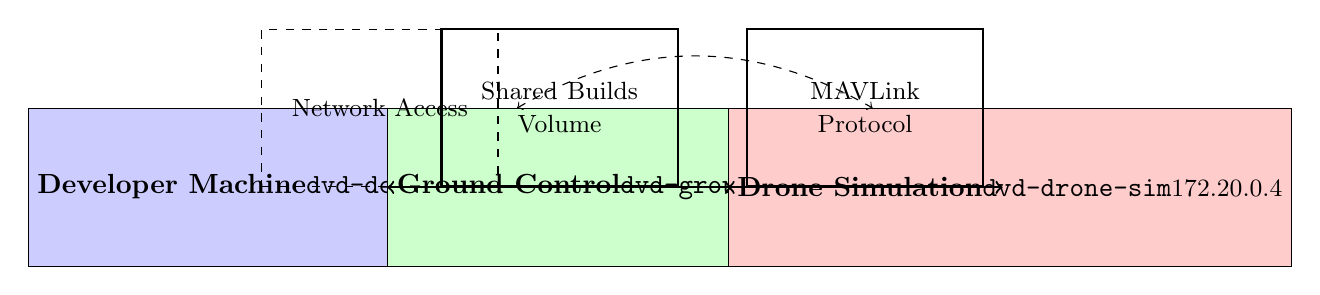
\begin{tikzpicture}[node distance=4cm, every node/.style={draw, rectangle, minimum width=3cm, minimum height=2cm, text centered}]
    
    % Define nodes
    \node (dev) [fill=blue!20] {
        \textbf{Developer Machine} \\
        \texttt{dvd-developer-machine} \\
        \small{172.20.0.2}
    };
    
    \node (gcs) [right of=dev, fill=green!20] {
        \textbf{Ground Control} \\
        \texttt{dvd-ground-control} \\
        \small{172.20.0.3}
    };
    
    \node (drone) [right of=gcs, fill=red!20] {
        \textbf{Drone Simulation} \\
        \texttt{dvd-drone-sim} \\
        \small{172.20.0.4}
    };
    
    % Define connections
    \draw[<->, thick] (dev) -- (gcs) node[midway, above, text width=2cm, text centered] {\small Shared Builds \\ Volume};
    \draw[<->, thick] (gcs) -- (drone) node[midway, above, text width=2cm, text centered] {\small MAVLink \\ Protocol};
    \draw[<->, dashed] (dev) to[bend left=30] (drone) node[midway, above] {\small Network Access};
    
\end{tikzpicture}
\caption{DVD Container-Topologie}
\end{figure}

\subsection{Netzwerkkonfiguration}

\begin{longtable}{|l|l|l|l|}
\caption{Netzwerk-Konfiguration der DVD-Container} \\
\hline
\textbf{Container} & \textbf{IP-Bereich} & \textbf{Exposed Ports} & \textbf{Protokoll} \\
\hline
\endfirsthead
\hline
\textbf{Container} & \textbf{IP-Bereich} & \textbf{Exposed Ports} & \textbf{Protokoll} \\
\hline
\endhead
\hline
\endfoot
\hline
\endlastfoot

Developer Machine & 172.20.0.2 & - & SSH, ICMP \\
Ground Control & 172.20.0.3 & 14550/udp, 5760/tcp & MAVLink, MAVProxy \\
Drone Simulation & 172.20.0.4 & 5762/tcp, 14551/udp & SITL, MAVLink \\
Network Bridge & 172.20.0.1 & - & Gateway \\
\end{longtable}

\section{Developer Machine Container}

\subsection{Zweck und Funktion}

Die Developer Machine dient als Einstiegspunkt für CTF-Teilnehmer und simuliert eine typische Entwicklungsumgebung mit gezielten Schwachstellen.

\subsection{Software-Stack}

\begin{lstlisting}[language=bash, caption=Installierte Pakete]
# Basis-System
FROM ubuntu:22.04

# Entwicklungstools
apt-utils curl iproute2 nano vim net-tools
iputils-ping python3 python3-pip wget git make g++

# Spezielle Pakete
expect cron sudo openssh-client build-essential

# Python-Bibliotheken
pip3 install future pymavlink MAVProxy mavsdk
\end{lstlisting}

\subsection{Benutzer-Konfiguration}

\begin{longtable}{|l|l|l|}
\caption{Benutzer-Accounts und Berechtigungen} \\
\hline
\textbf{Benutzer} & \textbf{Passwort} & \textbf{Berechtigungen} \\
\hline
\endfirsthead
\hline
\textbf{Benutzer} & \textbf{Passwort} & \textbf{Berechtigungen} \\
\hline
\endhead
\hline
\endfoot
\hline
\endlastfoot

developer & dev123 & sudo crontab (NOPASSWD) \\
root & - & Full administrative access \\
\end{longtable}

\subsection{Verzeichnisstruktur}

\begin{lstlisting}[language=bash, caption=Wichtige Verzeichnisse]
/home/developer/
├── Documents/
│   ├── README.txt          # CTF-Hinweise
│   └── known_issues.txt    # System-Dokumentation
├── projects/
│   └── drone_dev.py        # Entwicklungs-Skript
/opt/
├── shared-builds/          # Shared Volume
│   ├── return-to-land.py   # RTL-Komponente
│   └── flag.txt           # Challenge-Flag
└── build-update.sh        # Malicious Build Script
\end{lstlisting}

\section{Ground Control Station Container}

\subsection{Zweck und Funktion}

Die Ground Control Station überwacht Drohnenoperationen und stellt das Deployment-Target für kompromittierte Software-Komponenten dar.

\subsection{Monitoring-Mechanismus}

\begin{lstlisting}[language=bash, caption=Deploy-Monitor-Skript]
#!/bin/bash
# Monitor shared builds and deploy to ground control
while true; do
    if [ -f "/opt/shared-builds/return-to-land.py" ]; then
        echo "[GCS] Detected updated RTL module"
        cp /opt/shared-builds/return-to-land.py /return-to-land.py
        chmod +x /return-to-land.py
        echo "[GCS] RTL module deployed successfully"
    fi
    sleep 30
done
\end{lstlisting}

\subsection{MAVLink-Integration}

Das Ground Control System kommuniziert über das MAVLink-Protokoll mit der Drohnensimulation:

\begin{itemize}
    \item \textbf{Port 14550/udp:} Hauptkommunikationskanal
    \item \textbf{Port 5760/tcp:} MAVProxy-Interface
    \item \textbf{Protokoll:} MAVLink v2.0
    \item \textbf{Dialect:} ArduPilot Mega
\end{itemize}

\section{Drone Simulation Container}

\subsection{SITL-Konfiguration}

Die Drohnensimulation basiert auf ArduPilot SITL (Software In The Loop):

\begin{lstlisting}[language=bash, caption=SITL-Parameter]
# Umgebungsvariablen
SITL_SPEEDUP=1          # Real-time simulation
SITL_RATE=400           # 400Hz update rate

# Netzwerk-Konfiguration
SITL_PORT=5762          # TCP-Port für SITL
MAVLINK_PORT=14551      # UDP-Port für MAVLink
\end{lstlisting}

\subsection{Simulationsparameter}

\begin{longtable}{|l|l|l|}
\caption{Drohnen-Simulationsparameter} \\
\hline
\textbf{Parameter} & \textbf{Wert} & \textbf{Beschreibung} \\
\hline
\endfirsthead
\hline
\textbf{Parameter} & \textbf{Wert} & \textbf{Beschreibung} \\
\hline
\endhead
\hline
\endfoot
\hline
\endlastfoot

Vehicle Type & Quadcopter & Standard-Multirotor \\
Flight Controller & ArduCopter & ArduPilot-basiert \\
Physics Engine & JSBSim & Realistische Flugsimulation \\
Ground Speed & 0-20 m/s & Konfigurierbare Geschwindigkeit \\
Max Altitude & 120m AGL & Regulatorische Begrenzung \\
\end{longtable}

\section{Volume-Management}

\subsection{Persistente Volumes}

Das System nutzt drei persistente Docker-Volumes:

\begin{enumerate}
    \item \textbf{developer-home:} Persistierung von Entwicklerdateien
    \item \textbf{shared-builds:} Gemeinsamer Speicher für Build-Artefakte
    \item \textbf{drone-logs:} Sammlung von Flugdaten und Logs
\end{enumerate}

\subsection{Volume-Konfiguration}

\begin{lstlisting}[language=yaml, caption=Docker Compose Volume-Definition]
volumes:
  developer-home:
    driver: local
  shared-builds:
    driver: local
  drone-logs:
    driver: local
\end{lstlisting}

\section{Sicherheitsarchitektur}

\subsection{Intentionale Schwachstellen}

Das System enthält bewusst implementierte Schwachstellen für Bildungszwecke:

\begin{longtable}{|l|l|l|}
\caption{Implementierte Schwachstellen} \\
\hline
\textbf{Komponente} & \textbf{Schwachstelle} & \textbf{MITRE ATT\&CK} \\
\hline
\endfirsthead
\hline
\textbf{Komponente} & \textbf{Schwachstelle} & \textbf{MITRE ATT\&CK} \\
\hline
\endhead
\hline
\endfoot
\hline
\endlastfoot

Developer Machine & Sudo crontab NOPASSWD & T1053.003 \\
Shared Builds & Unsecured file permissions & T1222.002 \\
Build Process & No integrity verification & T1195.002 \\
Network & Unencrypted communication & T1040 \\
\end{longtable}

\subsection{Container-Isolation}

Trotz der intentionalen Schwachstellen sind die Container durch Docker-Mechanismen isoliert:

\begin{itemize}
    \item \textbf{Namespace-Isolation:} PID, Network, Mount, UTS
    \item \textbf{Cgroup-Limits:} Ressourcenbegrenzung
    \item \textbf{Seccomp-Profile:} Syscall-Filterung
    \item \textbf{User-Namespaces:} UID/GID-Mapping
\end{itemize}

\section{Deployment-Anweisungen}

\subsection{Systemanforderungen}

\begin{longtable}{|l|l|}
\caption{Minimale Systemanforderungen} \\
\hline
\textbf{Komponente} & \textbf{Anforderung} \\
\hline
\endfirsthead
\hline
\textbf{Komponente} & \textbf{Anforderung} \\
\hline
\endhead
\hline
\endfoot
\hline
\endlastfoot

CPU & 2+ Cores, 2.0+ GHz \\
RAM & 4+ GB verfügbar \\
Storage & 10+ GB freier Speicher \\
Docker & Version 20.10+ \\
Docker Compose & Version 2.0+ \\
OS & Linux/macOS/Windows \\
\end{longtable}

\subsection{Installation}

\begin{lstlisting}[language=bash, caption=System-Deployment]
# Repository klonen
git clone https://github.com/user/Damn-Vulnerable-Drone.git
cd Damn-Vulnerable-Drone

# Container-Images erstellen
docker-compose build

# System starten
docker-compose up -d

# Status überprüfen
docker-compose ps

# Zugriff auf Developer Machine
docker exec -it dvd-developer-machine /bin/bash
\end{lstlisting}

\subsection{Konfigurationsoptionen}

\begin{lstlisting}[language=bash, caption=Umgebungsvariablen]
# .env Datei erstellen
echo "COMPOSE_PROJECT_NAME=dvd" > .env
echo "NETWORK_SUBNET=172.20.0.0/16" >> .env
echo "SITL_SPEEDUP=1" >> .env
echo "LOG_LEVEL=INFO" >> .env
\end{lstlisting}

\section{Monitoring und Logging}

\subsection{Container-Logs}

\begin{lstlisting}[language=bash, caption=Log-Monitoring]
# Alle Container-Logs anzeigen
docker-compose logs -f

# Spezifische Container-Logs
docker-compose logs -f developer-machine
docker-compose logs -f ground-control-station
docker-compose logs -f damn-vulnerable-drone

# Log-Ausgabe in Datei
docker-compose logs > dvd-system.log
\end{lstlisting}

\subsection{Performance-Monitoring}

\begin{lstlisting}[language=bash, caption=Ressourcen-Überwachung]
# Container-Ressourcenverbrauch
docker stats

# Detaillierte Container-Information
docker inspect dvd-developer-machine

# Netzwerk-Analyse
docker network inspect dvd_dvd-network
\end{lstlisting}

\section{Wartung und Updates}

\subsection{Container-Updates}

\begin{lstlisting}[language=bash, caption=System-Updates]
# Container stoppen
docker-compose down

# Images neu erstellen
docker-compose build --no-cache

# System neu starten
docker-compose up -d

# Verwaiste Images entfernen
docker image prune -f
\end{lstlisting}

\subsection{Backup-Strategien}

\begin{lstlisting}[language=bash, caption=Volume-Backup]
# Volume-Backup erstellen
docker run --rm -v dvd_developer-home:/data \
  -v $(pwd):/backup ubuntu tar czf \
  /backup/developer-home-backup.tar.gz -C /data .

# Volume-Restore
docker run --rm -v dvd_developer-home:/data \
  -v $(pwd):/backup ubuntu tar xzf \
  /backup/developer-home-backup.tar.gz -C /data
\end{lstlisting}

\section{Troubleshooting}

\subsection{Häufige Probleme}

\subsubsection{Container-Start-Probleme}

\begin{lstlisting}[language=bash, caption=Container-Debugging]
# Container-Status überprüfen
docker-compose ps

# Container-Logs analysieren
docker-compose logs container-name

# Manuelle Container-Erstellung
docker-compose up --force-recreate container-name
\end{lstlisting}

\subsubsection{Netzwerk-Konnektivitätsprobleme}

\begin{lstlisting}[language=bash, caption=Netzwerk-Debugging]
# Netzwerk-Konfiguration überprüfen
docker network ls
docker network inspect dvd_dvd-network

# Container-Netzwerk-Interfaces
docker exec container-name ip addr show

# Ping-Tests zwischen Containern
docker exec dvd-developer-machine ping -c 3 ground-control
\end{lstlisting}

\subsubsection{Volume-Mount-Probleme}

\begin{lstlisting}[language=bash, caption=Volume-Debugging]
# Volume-Information anzeigen
docker volume ls
docker volume inspect dvd_shared-builds

# Volume-Permissions überprüfen
docker exec dvd-developer-machine ls -la /opt/shared-builds/

# Volume-Cleanup bei Problemen
docker volume prune
\end{lstlisting}

\section{Erweiterungsmöglichkeiten}

\subsection{Zusätzliche Schwachstellen}

Das System kann um weitere Angriffsvektoren erweitert werden:

\begin{itemize}
    \item \textbf{Web-Interface:} Vulnerable Admin-Panel
    \item \textbf{Database:} SQL-Injection-Scenarios
    \item \textbf{API-Endpoints:} REST-API-Schwachstellen
    \item \textbf{IoT-Devices:} Sensor-Network-Kompromittierung
\end{itemize}

\subsection{Multi-Drone-Scenarios}

\begin{lstlisting}[language=yaml, caption=Erweiterte Drohnen-Flotte]
# Zusätzliche Drohnen-Services
drone-02:
  build:
    context: .
    dockerfile: damn-vulnerable-drone/Dockerfile
  container_name: dvd-drone-02
  ports:
    - "5763:5762/tcp"
    - "14552:14551/udp"
\end{lstlisting}

\section{Sicherheitshinweise}

\subsection{Produktionsumgebung}

\textbf{WARNUNG:} Dieses System ist ausschließlich für Bildungszwecke konzipiert und enthält bewusste Sicherheitslücken. Es darf NIEMALS in Produktionsumgebungen eingesetzt werden.

\subsection{Isolation-Empfehlungen}

\begin{itemize}
    \item Betrieb in isolierten Netzwerken oder VMs
    \item Keine Verbindung zu kritischen Systemen
    \item Regelmäßige Überprüfung der Container-Isolation
    \item Monitoring von Host-System-Aktivitäten
\end{itemize}

\section{Literaturverzeichnis}

\begin{itemize}
    \item MITRE ATT\&CK Framework: \url{https://attack.mitre.org/}
    \item Docker Security Best Practices: \url{https://docs.docker.com/engine/security/}
    \item ArduPilot Documentation: \url{https://ardupilot.org/dev/}
    \item MAVLink Protocol: \url{https://mavlink.io/en/}
    \item Container Security Standards: \url{https://www.nist.gov/publications/}
\end{itemize}

\end{document}